\section{Experiments}
\label{sec:exp}
We evaluate the efficiency and usefulness of \framework\ in an extensive set of experiments. We consider two types of experiments: first, a performance study to measure the influence of relevance, size constraint $k$, and time limit on execution time, and second, a user study to evaluate how efficient analysts can gain insights in our framework.

\vspace{5pt}
\noindent {\bf Experiment Settings.} Unless otherwise stated, we use the same settings discussed in Section \ref{sec:scenarios}. All experiments are implemented in Python (functionality) and JavaScript (visualization) on a 2.4GHz Intel Core i5 machine with an 8GB main memory, running OS X 10.9.2.

\begin{figure}
  \centering
  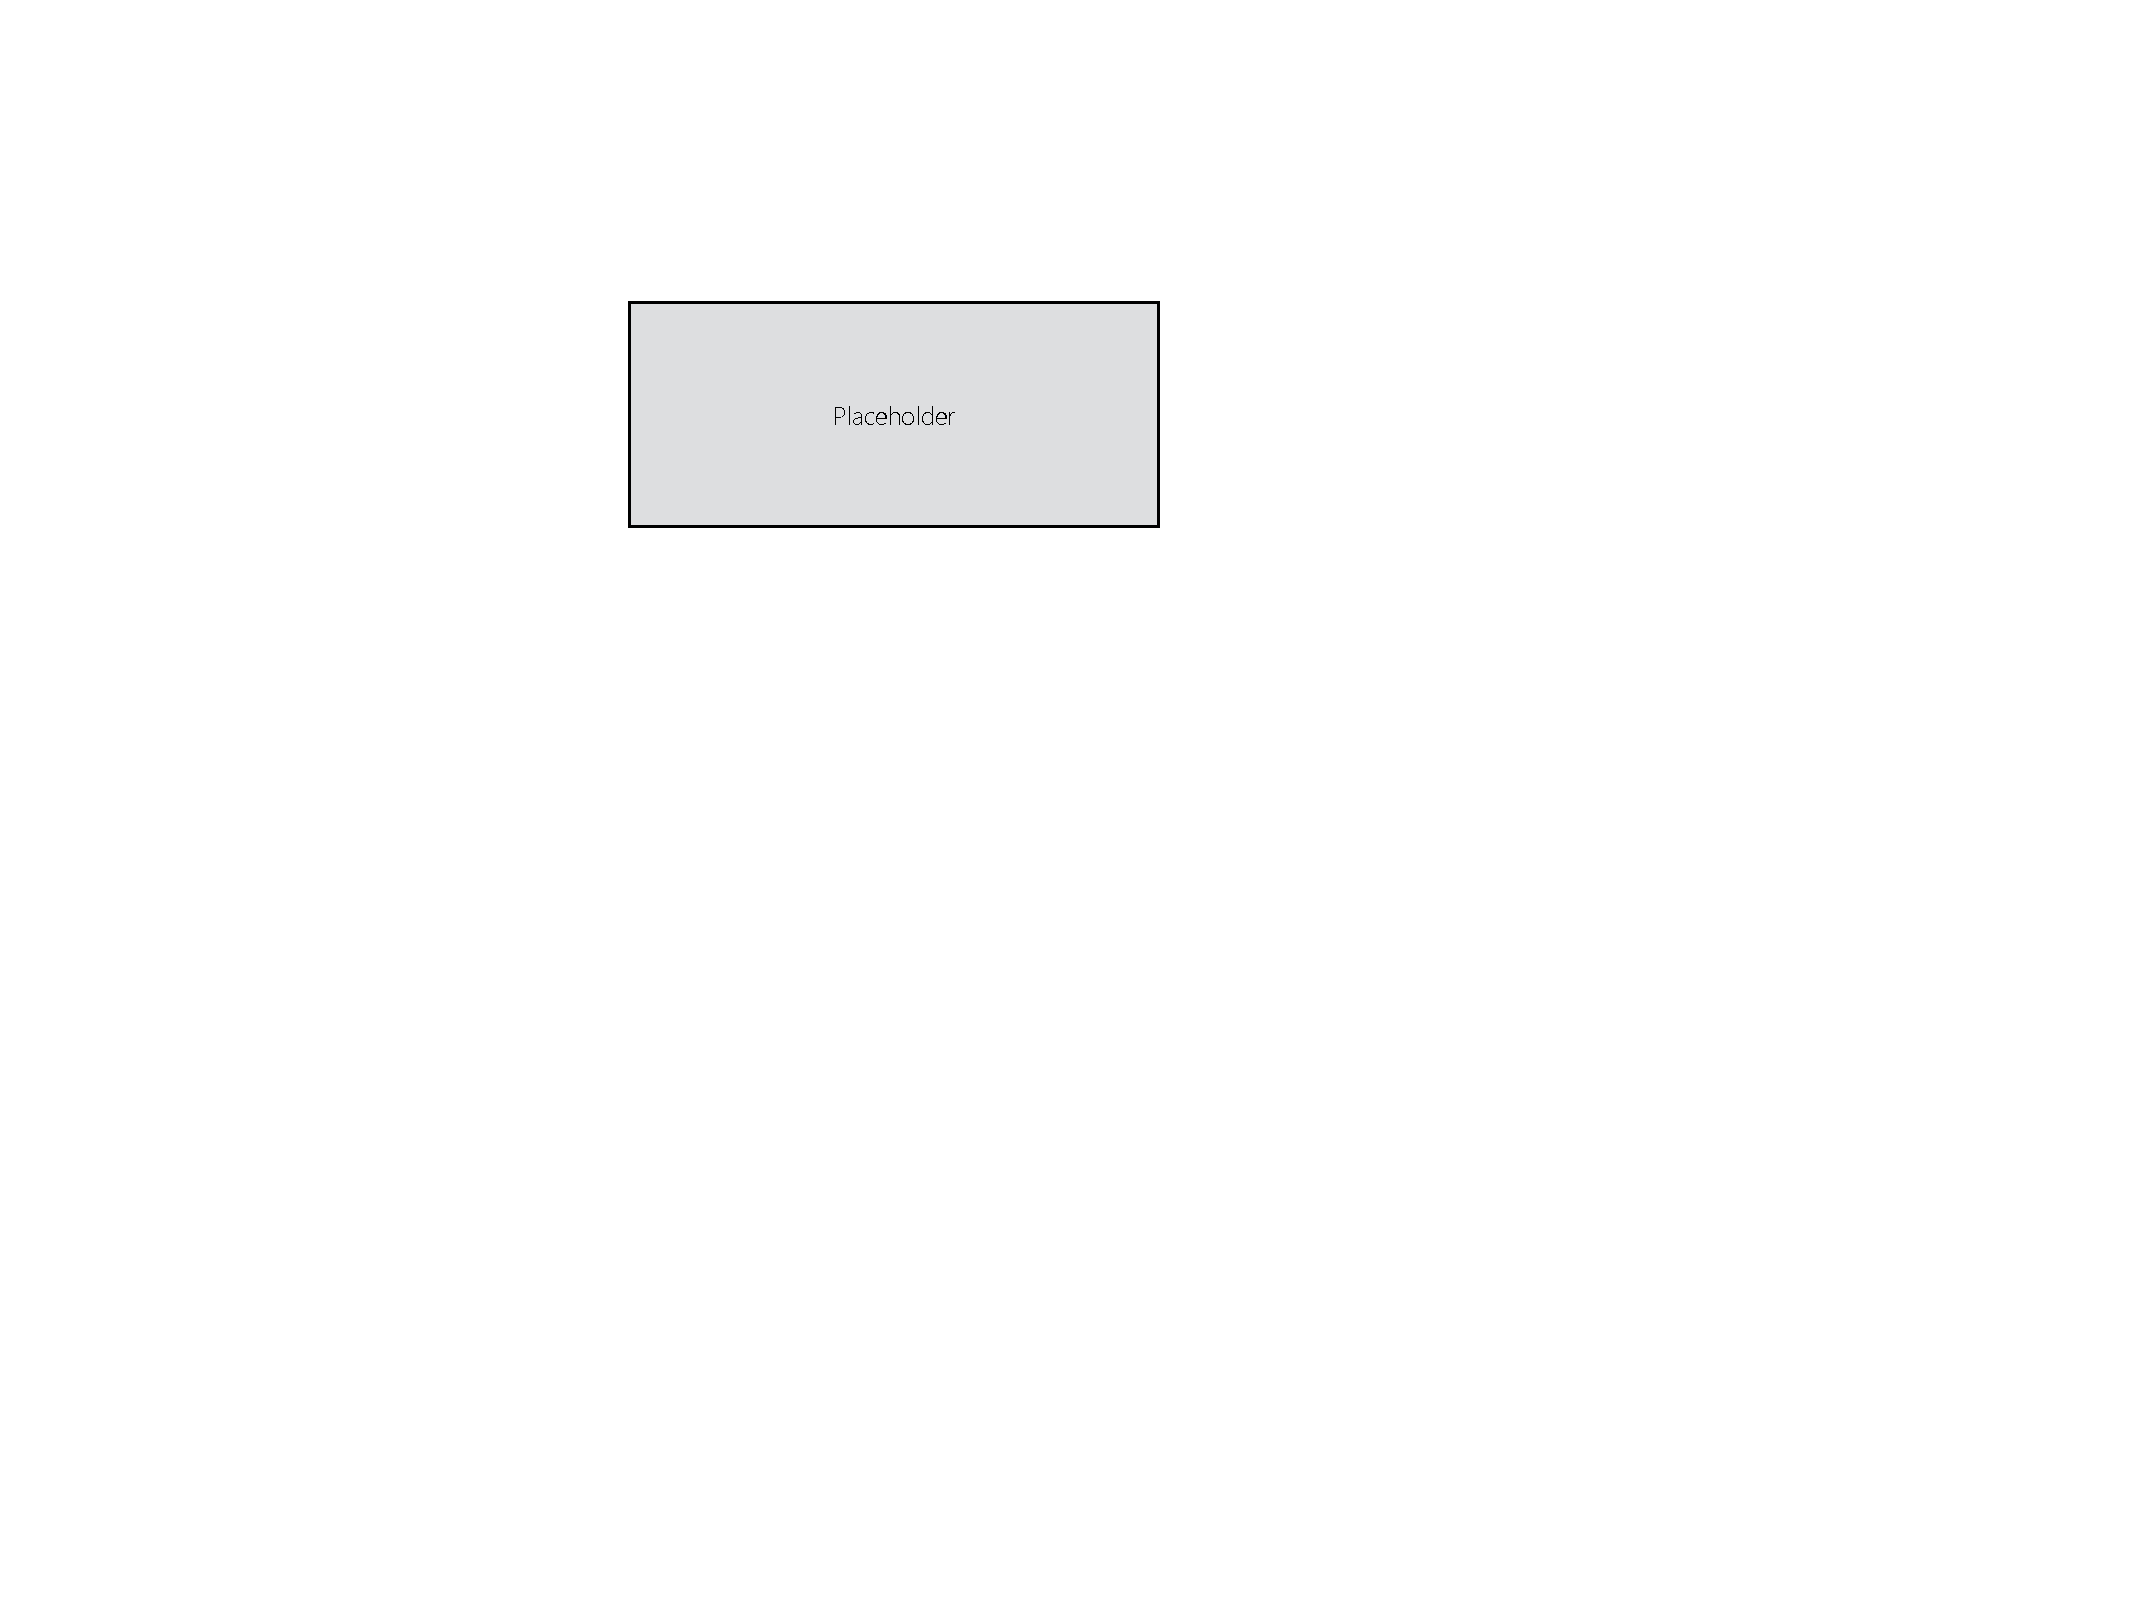
\includegraphics[width=\columnwidth]{figs/placeholder}
\caption{Performance Evaluation}
\label{fig:performance}
\end{figure}

\vspace{5pt}
\noindent {\bf Performance Study.} \framework\ is designed for exploratory context where interactivity is a need. The ``best-effort'' greedy approach of {\sc Highlighter} (Algorithm \ref{algo:geoh}) guarantees to return the best possible results within a time limit. We consider a large time limit ($tlimit = 10s$) in order to evaluate the effect of relevance and size constraint ($k$) on execution time.
% Figure \ref{fig:performance} illustrates the results by measuring the execution time.

Figure \ref{fig:performance} left illustrates the effect of size constraint by varying $k$ from $2$ to $500$. We observe that \colorred{[observation based on experiment results]}. Figure \ref{fig:performance} right illustrates the effect of relevance threshold by varying $\sigma$ from $0.1$ to $1.0$. We observe that \colorred{[observation based on experiment results]}.

\vspace{5pt}
\noindent {\bf User Study.}
The principled question that we ask ourselves is whether \framework\ is useful for analyst in practice. To answer this question, we designed a user study with $24$ participants. Half of the participants know the New York region well (experts) and the other half have a limited knowledge (novice). In our user study, we define a task for each participant and ask him/her to fulfill the task using \framework\ framework and {\sc Tableau}. Then we measure the cardinality of steps to reach the goal.

\begin{figure}
  \centering
  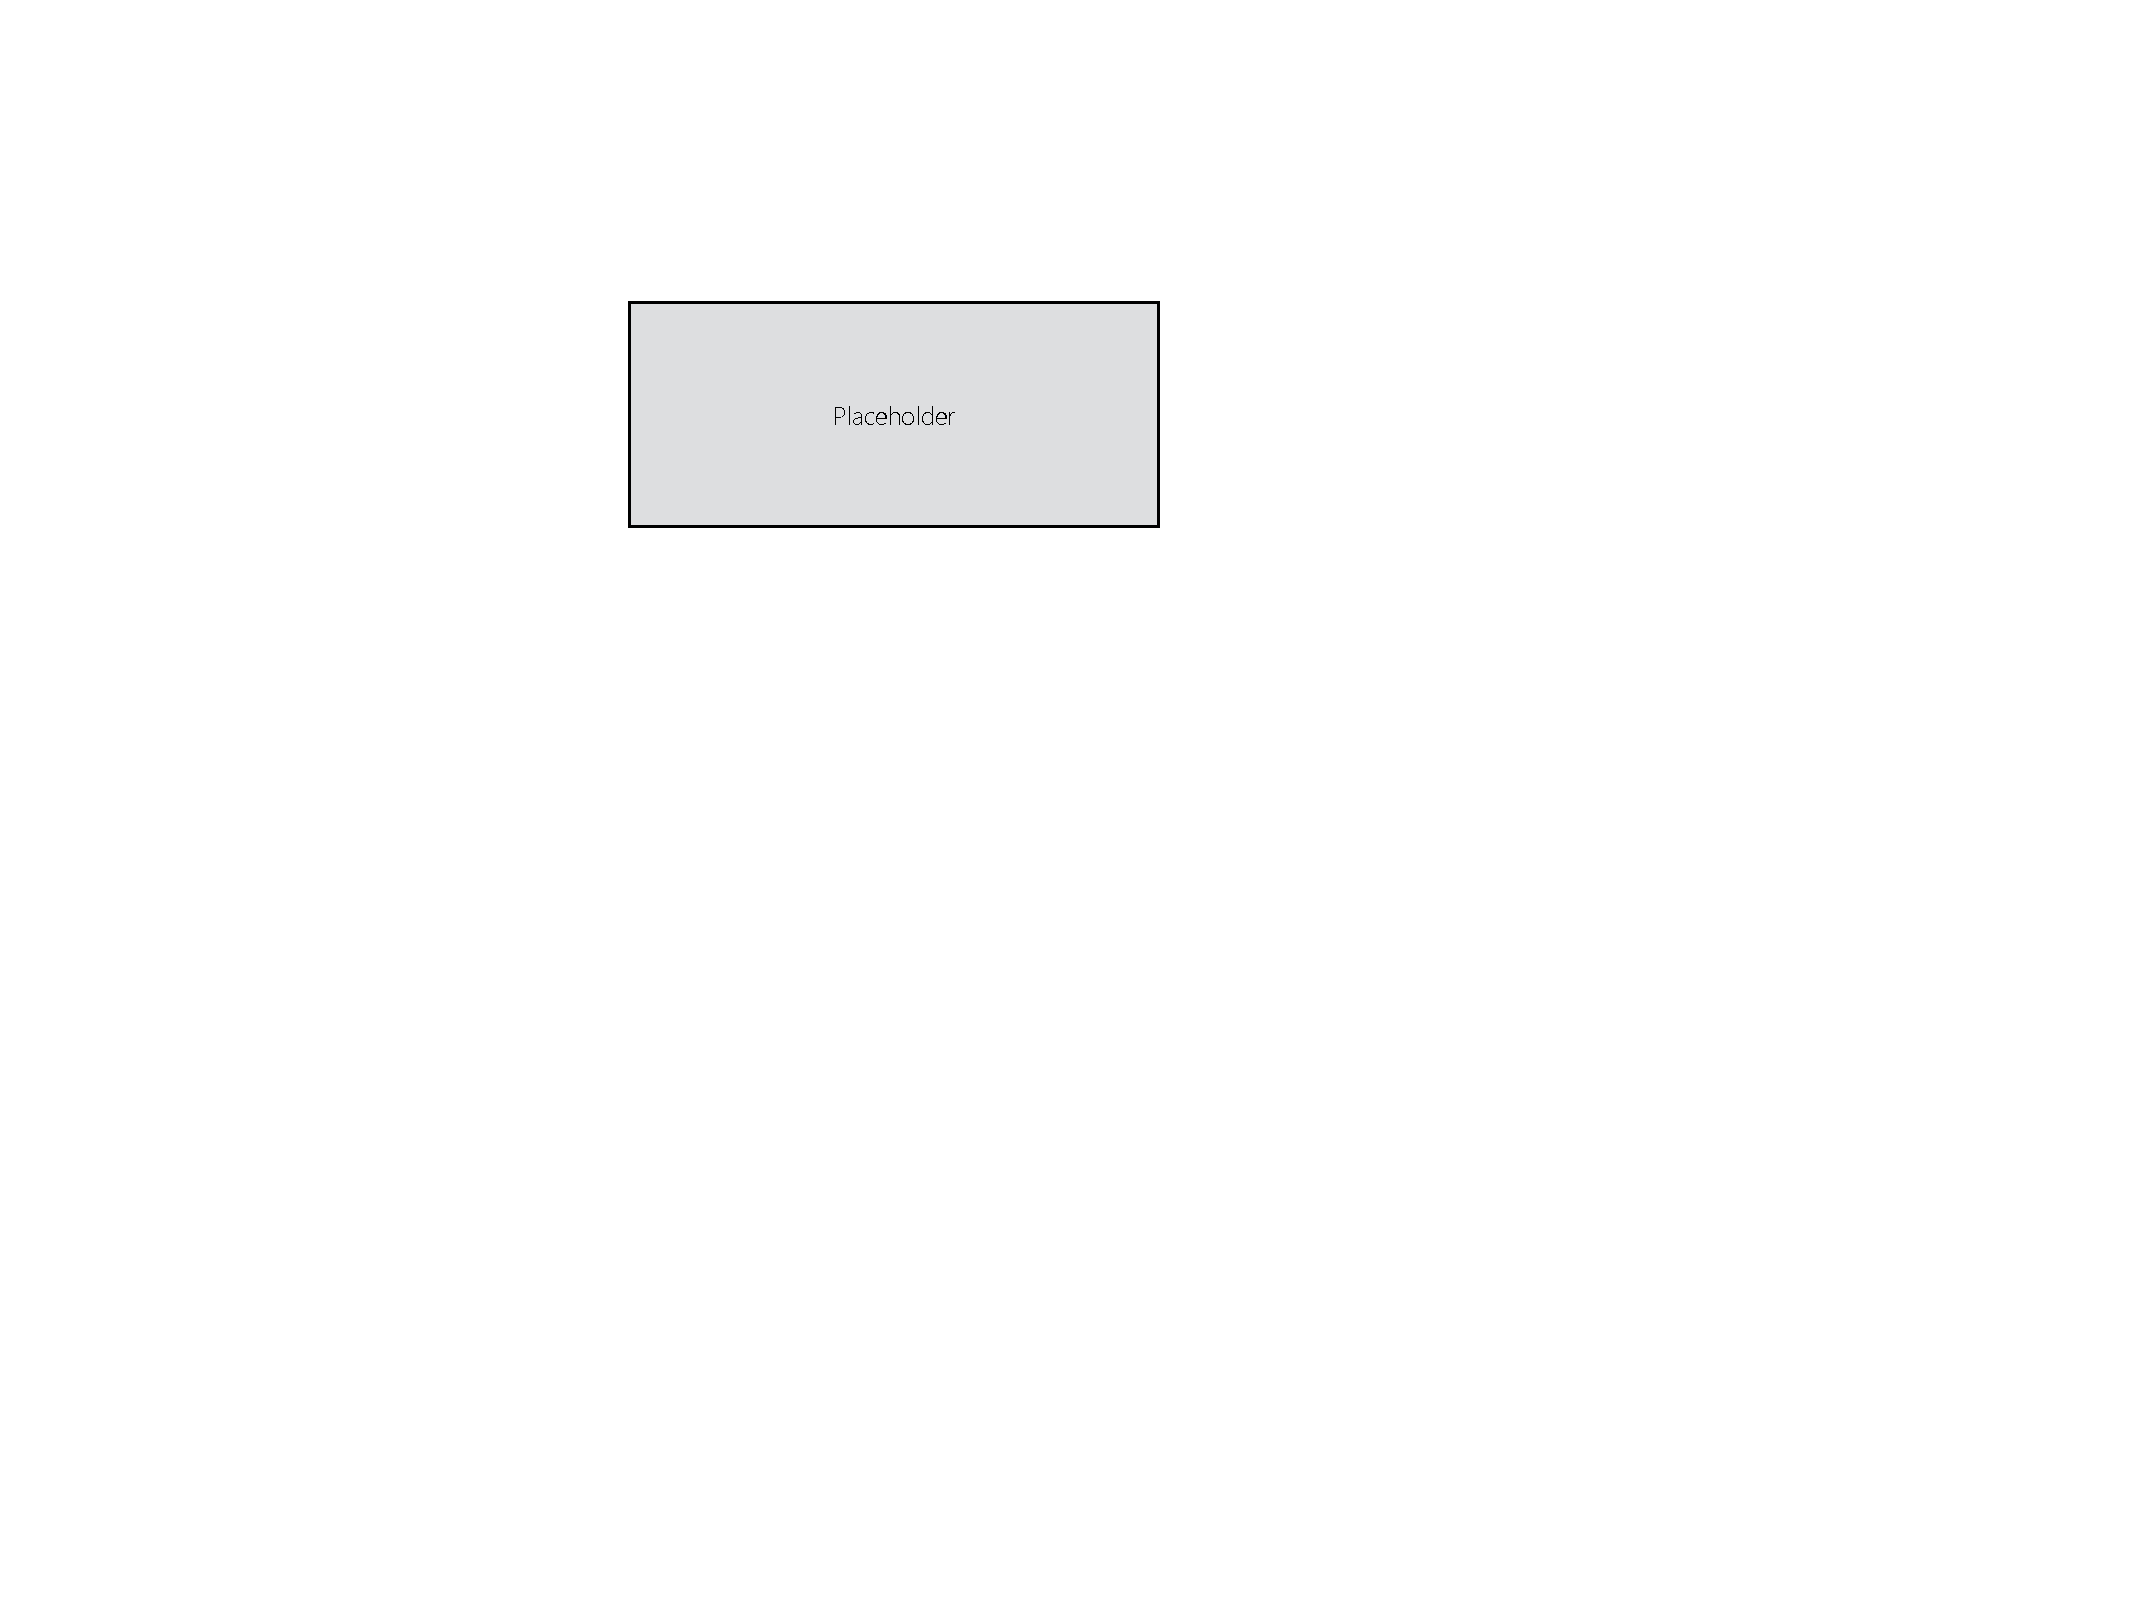
\includegraphics[width=\columnwidth]{figs/placeholder}
\caption{User Study}
\label{fig:userstudy}
\end{figure}

We define two tasks, {\em T1: finding a point in a requested location}, and {\em T2: finding a point with a requested profile}. As an example for {\em T1}, we ask participants to find points in the Central Park area. An example of {\em T2} is to find a drop-off point with \$2 tip whose trip distance is 3 miles. Participants may begin their navigation from three different starting points: {\em I1: close to the goal}, {\em I2: far from the goal}, and {\em I3: random}. We evaluate the effect of expertise, goal and starting point on the analysis length. Figure \ref{fig:userstudy} illustrates the results.

We observe that in general, \colorred{it takes XXX steps to reach a defined goal} in \framework. Level of expertise improves \colorred{the analysis length in average by XXX step}. This shows that the guidance components help analysts discover their data and quickly reach to the goal. Interestingly, starting points do not have a huge influence. It is potentially due to the diversity component which provides distinct options. We also observe that {\em T2} is an easier task than {\em T1}. This is potentially due to similarity component where the analyst can request options similar to what she has already seen and greedily moves to match profiles.

We also asked our participants about their insights on \framework. We ask them to rate the following metric on a 5-star scale: {\em usefulness} and {\em ease-of-use}. In summary, we found that \colorred{[explain received results]}.